\documentclass[num-refs]{wiley-article}

\usepackage{graphicx}
\usepackage[space]{grffile}
\usepackage{latexsym}
\usepackage{textcomp}
\usepackage{longtable}
\usepackage{tabulary}
\usepackage{booktabs,array,multirow}
\usepackage{amsfonts,amsmath,amssymb}
\usepackage{natbib}
\usepackage{url}
\usepackage{hyperref}
\hypersetup{colorlinks=false,pdfborder={0 0 0}}
%\usepackage{etoolbox}
%\makeatletter
%\patchcmd\@combinedblfloats{\box\@outputbox}{\unvbox\@outputbox}{}{%
%  \errmessage{\noexpand\@combinedblfloats could not be patched}%
%}%
%\makeatother
% You can conditionalize code for latexml or normal latex using this.
\newif\iflatexml\latexmlfalse
\providecommand{\tightlist}{\setlength{\itemsep}{0pt}\setlength{\parskip}{0pt}}%

\AtBeginDocument{\DeclareGraphicsExtensions{.pdf,.PDF,.eps,.EPS,.png,.PNG,.tif,.TIF,.jpg,.JPG,.jpeg,.JPEG}}

\usepackage[utf8]{inputenc}
\usepackage[english]{babel}

% Add any additional LaTeX packages and macros here
\usepackage{siunitx}
\usepackage{placeins}

%---

\iflatexml
% Add any LateXML specific commands here

%---

\else
% The commands below will only change the exported PDF. Edit or remove as needed

\paperfield{Clinical Neurology}
\abbrevs{GLMM, generalized linear mixed model; IRT, item response theory; KSS, Kahneman-Sibony-Sunstein; MCMC, Markov chain Monte Carlo; SSIT, similar skill individual threshold.}
\corraddress{M. Brandon Westover MD PhD, Department of Neurology, Massachusetts General Hospital, Harvard Medical School, Boston, MA, USA}
\corremail{mwestover@mgh.harvard.edu}
\fundinginfo{National Institutes of Health, Grant/Award Numbers: R01AG073410, R01HL161253, R01NS126282, R01AG073598, R01NS131347, R01NS130119}
\fi

%---

\papertype{Original Article}

\title{Measuring Skill and Noise in Medical Decisions}

\author[1]{M. Brandon Westover}
\affil[1]{Harvard Medical School}

\author[2]{Fabio Nascimento}
\affil[2]{Washington University School of Medicine in St. Louis}

\author[1]{Jin Jing}
\affil[1]{Harvard Medical School}

\runningauthor{M. Brandon Westover}

\begin{document}

\maketitle
\selectlanguage{english}
\begin{abstract}
\textbf{Background:} When multiple clinicians evaluate the same cases, disagreement arises from various forms of noise: systematic bias (level noise), idiosyncratic case-by-rater interactions (pattern noise), and within-rater inconsistency (occasion noise). The observed variation in responses across cases reflects both the underlying signal (genuine differences in case difficulty) and these noise sources. Traditional reliability metrics collapse all disagreement into a single number, preventing identification of specific noise sources.

\textbf{Methods:} We present a unified statistical framework for decomposing variation in binary medical decisions. We show that Item Response Theory (IRT), signal detection theory (SSIT), and the Kahneman-Sibony-Sunstein (KSS) noise decomposition are special cases of a generalized linear mixed model. We use Bayesian estimation via Markov chain Monte Carlo to obtain posterior distributions for all variance components and their relative contributions. We demonstrate the approach using data from epilepsy diagnosis and EEG spike classification.

\textbf{Results:} In an epilepsy diagnosis study with 20 expert neurologists reviewing 50 cases on two occasions, system noise (level + pattern + occasion) accounted for 31-34\% of total variation. Based on clinical history alone, level noise (systematic bias) was the dominant component (23\%). After incorporating EEG and neuroimaging results, pattern noise (idiosyncratic case interpretations) became dominant (24\%), while level noise decreased to 5\%. Occasion noise remained minimal (1\%) despite 16\% of cases showing diagnostic reversals between occasions. Diagnostic accuracy was 71\% overall, but only 56\% for difficult cases.

\textbf{Conclusions:} The noise decomposition framework provides actionable insights into sources of diagnostic disagreement. By separating level, pattern, and occasion noise, researchers can design targeted interventions (e.g., threshold calibration for level noise, case-based training for pattern noise, decision aids for occasion noise). We provide practical guidance on sample size requirements, model implementation, and interpretation for applied medical researchers.

\textbf{Keywords} --- inter-rater reliability, noise decomposition, item response theory, signal detection theory, generalized linear mixed models, Bayesian hierarchical models, diagnostic disagreement%
\end{abstract}%




\section*{Introduction}

{\label{707961}}

Medical decision-making often involves expert judgment calls where different clinicians may disagree. Understanding the sources of this disagreement is important for improving diagnostic reliability and accuracy, designing training programs, and determining appropriate study sample sizes. When multiple experts rate the same cases, disagreement between raters on individual cases arises entirely from noise, while variation in responses across different cases reflects the underlying signal (genuine differences in case difficulty) plus these noise sources.

Traditional reliability metrics such as Cohen's kappa or intraclass correlation coefficients tell us \textit{how much} experts disagree, but not \textit{why}. A kappa of 0.65 indicates moderate agreement, but provides no insight into whether disagreement stems from differing personal thresholds, idiosyncratic interpretations of evidence, or random inconsistency. Without understanding the sources of disagreement, we cannot design targeted interventions to improve reliability.

Recent work in decision science~\cite{Kahneman2021} has identified distinct types of noise: \textit{level noise} (systematic differences in how lenient or stringent raters are), \textit{pattern noise} (idiosyncratic differences in how raters weigh features of individual cases), and \textit{occasion noise} (inconsistency within the same rater across repeated assessments). Crucially, each noise type suggests different remedies: level noise calls for threshold calibration, pattern noise for case-based training, and occasion noise for decision support tools.

\textbf{Framing diagnosis as a measurement problem.} Consider two neurologists who disagree on whether a patient has epilepsy. Is the disagreement because one expert is generally more conservative in diagnosing epilepsy (level noise), or because they interpret the same EEG spike differently (pattern noise), or because one expert is having an off day (occasion noise)? Traditional metrics cannot answer this question. This paper provides a "diagnostic tool for diagnostic systems"---a framework to decompose disagreement into actionable components.

We present a unified statistical framework for quantifying these sources of variation in binary medical decisions. We show how Item Response Theory (IRT), signal detection theory, and the Kahneman-Sibony-Sunstein (KSS) noise decomposition framework can all be understood as special cases of a single generalized linear mixed model (GLMM). We demonstrate the framework using data from 20 expert neurologists diagnosing epilepsy, revealing that the dominant source of noise shifts depending on the available diagnostic information. We provide practical guidance for applied researchers on how to implement these models, interpret the results, and design studies to estimate noise components reliably.

\subsection*{Overview: Inputs, Outputs, and Use Cases}

To orient applied readers, we first summarize what this method requires, what it produces, and when it is useful.

\begin{table}[h!]
\centering
\small
\begin{tabular}{p{0.25\textwidth}p{0.65\textwidth}}
\toprule
\textbf{Component} & \textbf{Description} \\
\midrule
\multicolumn{2}{l}{\textbf{INPUTS}} \\
Binary ratings & Response array $Y_{ijt}$: ratings from $M$ raters on $N$ cases, optionally repeated over $T$ occasions \\
Sample sizes & Typical: $N \geq 30$ cases, $M \geq 10$ raters; $T \geq 2$ occasions if estimating occasion noise \\
Gold standard (optional) & Reference labels for evaluating accuracy (sensitivity/specificity); not required for noise decomposition \\
\midrule
\multicolumn{2}{l}{\textbf{PRIMARY OUTPUTS}} \\
Variance components & Standard deviations $\sigma_c, \sigma_\ell, \sigma_p, \sigma_o$ quantifying signal, level noise, pattern noise, and occasion noise \\
Percent contributions & Proportion of total variation explained by each component \\
Uncertainty & Credible intervals (Bayesian) or confidence intervals (frequentist) for all estimates \\
\midrule
\multicolumn{2}{l}{\textbf{SECONDARY OUTPUTS}} \\
Rater-level summaries & Individual bias ($\ell_j$), pattern consistency, occasion stability \\
Case-level summaries & Predicted consensus probability for each case \\
Model validation & Posterior predictive checks, goodness-of-fit diagnostics \\
\midrule
\multicolumn{2}{l}{\textbf{USE CASES}} \\
1. Quantify disagreement & Separate signal from noise; identify dominant noise sources \\
2. Compare groups & Test whether experts vs. novices differ in level, pattern, or occasion noise \\
3. Design studies & Determine required sample sizes (cases, raters, repeats) for target precision \\
4. Evaluate training & Measure changes in noise components before/after training interventions \\
5. Quality assurance & Identify raters with excessive bias or inconsistency \\
\bottomrule
\end{tabular}
\caption{Summary of inputs, outputs, and use cases for the noise decomposition framework.}
\label{tab:overview}
\end{table}

\subsection*{Why Decomposition Matters: An Illustrative Example}

Figure~\ref{fig:killer} illustrates why decomposing noise into its components is clinically valuable. We simulated two raters with \textit{identical} overall accuracy (sensitivity = 0.80, specificity = 0.80), but with different underlying noise profiles:

\begin{itemize}
    \item \textbf{Rater A ("Biased but Consistent"):} High level noise ($\sigma_\ell = 1.5$), low pattern noise ($\sigma_p = 0.3$), low occasion noise ($\sigma_o = 0.2$). This rater systematically over-calls (positive bias), but responds consistently to the same case across occasions and agrees with other biased raters.

    \item \textbf{Rater B ("Unbiased but Erratic"):} Low level noise ($\sigma_\ell = 0.3$), high pattern noise ($\sigma_p = 1.2$), high occasion noise ($\sigma_o = 0.8$). This rater has no systematic bias but responds idiosyncratically to individual cases and inconsistently across occasions.
\end{itemize}

Despite identical sensitivity and specificity, the heatmaps of responses (cases × occasions) look different. Rater A shows systematic patterns (all cases shifted upward), while Rater B shows scattered disagreements.

\textbf{Clinical implications:}
\begin{itemize}
    \item For Rater A: Threshold recalibration (e.g., show examples of borderline cases) could improve accuracy
    \item For Rater B: Case-based training (to reduce pattern noise) and decision aids (to reduce occasion noise) are needed
    \item Traditional metrics (kappa, accuracy) cannot distinguish these scenarios
\end{itemize}

\begin{figure}[h!]
\begin{center}
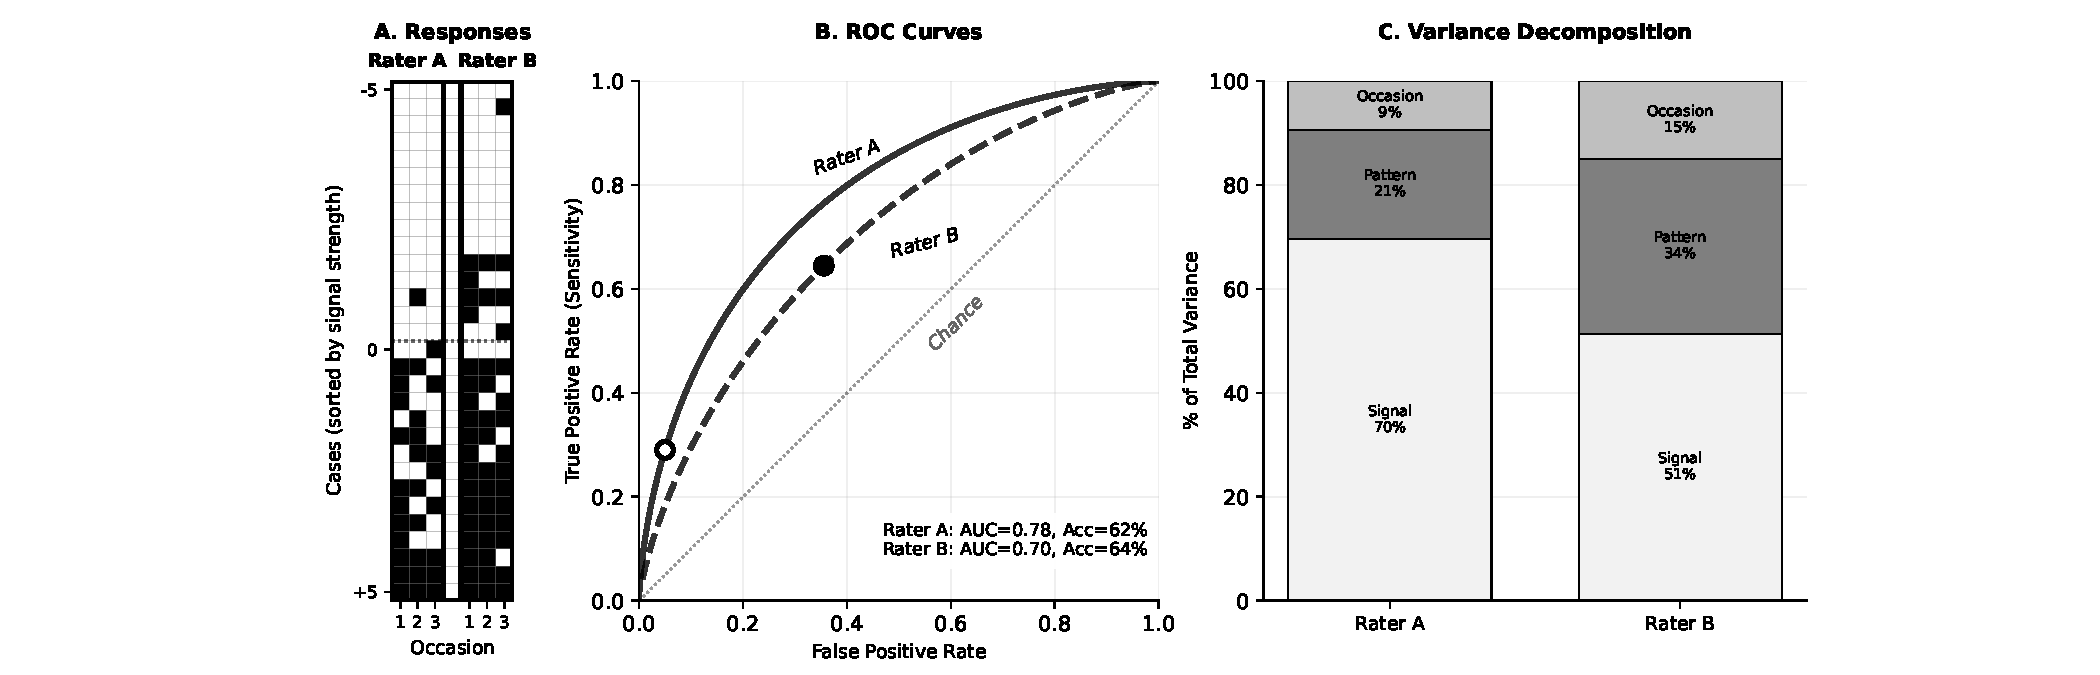
\includegraphics[width=1.0\textwidth]{killer_figure.pdf}
\caption{\textbf{Identical accuracy, different noise profiles.} Two simulated raters with similar overall performance but different noise decompositions. \textbf{Left (Rater A):} High level noise (systematic bias, $\sigma_\ell = 1.5$, 95\% of noise) but low pattern ($\sigma_p = 0.3$, 4\%) and occasion noise ($\sigma_o = 0.2$, 2\%), resulting in consistent but shifted responses. The heatmap shows clear horizontal banding. \textbf{Right (Rater B):} Low level noise ($\sigma_\ell = 0.3$, 4\%) but high pattern ($\sigma_p = 1.2$, 66\%) and occasion noise ($\sigma_o = 0.8$, 29\%), resulting in erratic, inconsistent responses. The heatmap shows scattered disagreements. \textbf{Top row:} Heatmaps of responses (30 cases × 3 occasions; red=negative, blue=positive; cases sorted by true probability; green dashed line = true positive/negative boundary). \textbf{Middle:} ROC curves showing similar performance. \textbf{Bottom:} Variance decomposition showing different noise sources. Despite similar overall accuracy, the appropriate interventions differ: threshold recalibration for Rater A vs. case-based training and decision support for Rater B. This illustrates why decomposing noise into its components is useful for designing effective interventions.}
\label{fig:killer}
\end{center}
\end{figure}

\begin{figure}[h!]
\begin{center}
\includegraphics[width=0.70\columnwidth]{Fig3-KSS-Model.png}
\caption{{\textbf{Noise decomposition: KSS framework} (A) Results from decomposing expert response data about cases histories in patients with suspected epilepsy. Variation in expert responses is decomposed into signal (information intrinsic to the cases), and system noise. System noise is further decomposed into level noise, pattern noise, and occasion noise. These different types of noise are combined additively with the signal to reach a final decision. The heatmaps show the actual estimates. (B) Quantitative summary of relative contributions of signal and noise to total variation in responses. Noise and signal levels are quantified by fitting normal distributions to the raw data to estimate standard deviations. The stacked bar plots show the relative contributions of the signal and noise levels. CN, consensus variation (signal level); LN, level noise; PN, pattern noise; ON, “occasion noise”. 
{\label{Fig3-KSS}}%
}}
\end{center}
\end{figure}

\begin{figure}[h!]
\begin{center}
\includegraphics[width=0.40\columnwidth]{Fig4-GoF.png}
\caption{{\textbf{Goodness of fit analysis} These plots show the relationship between observed quantities based on the raw expert responses data (x-axis) and the fitted model (y-axis) for signal, level noise, and pattern noise. Fits are excellent, as indicated by tight clustering of the data along the diagonal line. Results for occasion noise are not shown, because the process was different. 
{\label{Fig4-GoF}}%
}}
\end{center}
\end{figure}


\par\null

\section*{Three models of noise and skill}\label{3-models}

\subsection*{Notation}
Throughout this paper we use consistent notation:
\begin{itemize}
    \item $i = 1,\ldots,N$ indexes cases (e.g., patient records, candidate waveforms)
    \item $j = 1,\ldots,M$ indexes raters or experts
    \item $t = 1,\ldots,T$ indexes occasions (repeated ratings of the same case by the same rater)
    \item $Y_{ijt}$ is the binary response (0 or 1) from rater $j$ on case $i$ at occasion $t$
\end{itemize}

We now explain the IRT, SSIT, and KSS models. All three models have this form: $Pr(Y_{ijt}=1) = f(z'_{ijt})$, where $z'_{ijt} = c_i + \ell_j + n_{ijt}$. Here, $Y_{ijt}=1$ represents a 'yes', 'positive', or 'correct' answer, depending on the context. The function $f$ can be either the logistic function $f(x) = 1/[1+\exp(-x)]$, or the cumulative Gaussian (probit) function $f(x) = (2\pi)^{-1/2}\int_{-\infty}^x \exp(-u^2/2)du$. The components of $z'_{ijt}$ have somewhat different interpretations in the three models, which we explain below.

\subsection*{Item response theory (IRT) Rasch model}\label{section-IRT}
The most commonly used IRT model is the 1PL or Rasch model, in which $$z'_{ijt} = c_i+\ell_j.$$ In the context of our noise decomposition framework, we interpret $Pr(Y_{ijt}=1)$ as the probability of answering 'yes' or classifying case $i$ as 'class 1' (as opposed to 'class 0'). Under this interpretation, $c_i$ represents the signal strength or evidence level of the case, and $\ell_j$ represents rater $j$'s bias---the tendency to say 'yes' regardless of the signal. Note that in this model, $n_{ijt}=0$ and the model does not include pattern or occasion noise.

Note that the model for $z'_{ijt}$ does not depend on $t$: responses are assumed to depend only on case properties and rater characteristics. According to the 1PL model, the same rater will give the same response to the same case on different occasions. 

\subsection*{Similar skill individual threshold (SSIT)}\label{section-SSIT}
In the SSIT model,
\begin{eqnarray*}
  z'_{ijt} &=& c_i + n_{ijt} \\
  Y_{ijt}&=&\begin{cases}
    1, & \text{if $z'_{ijt}>\ell_j$}\\
    0, & \text{if $z'_{ijt}\leq \ell_j$},
  \end{cases}
\end{eqnarray*}
where $c_i$ is the signal strength for case $i$ and $n_{ijt}$ is the noise. For an ideal observer, $z'_{ijt} = c_i$, i.e., there is no noise ($n_{ijt}=0$). As indicated, decisions about the value of $Y_{ijt}$ are reached by comparing $z'_{ijt}$ with a threshold value $\ell_j$ that is particular to rater $j$.

Note that a mathematically equivalent formulation is
\begin{eqnarray*}
  z'_{ijt} &=& c_i + \ell_j + n_{ijt} \\
  Y_{ijt}&=&\begin{cases}
    1, & \text{if $z'_{ijt}>0$}\\
    0, & \text{if $z'_{ijt}\leq 0$},
  \end{cases}
\end{eqnarray*}
where we have absorbed $\ell_j$ into $z'_{ijt}$. This form is consistent with the KSS model (see below) and with the logistic GLMM formulation where $\text{Pr}(Y_{ijt}=1) = f(c_i + \ell_j + n_{ijt})$.

In SSIT, $\ell_j$ represents the decision threshold of rater $j$: the minimum evidence level at which that rater is willing to classify a case as positive. The noise $n_{ijt}$ represents uncertainty in the rater's perception or decision-making process. The noise is assumed to have a Gaussian distribution with zero mean and standard deviation $\sigma_j$. We refer to the inverse of the noise standard deviation as the rater's 'skill' level, $s_j = 1/\sigma_j$, so that higher skill (smaller $\sigma_j$) means the rater is closer to the ideal observer.

'Similar skill' in the SSIT name refers to the hypothesis that raters with similar levels of training tend to have the same skill level, so that a single skill (or inverse noise) parameter describes responses for all raters in a group: $s_j = s$, $\sigma_j = \sigma_s$.

\subsubsection*{ROC curves, skill, and noise in SSIT}\label{section-ROC}
When working with the SSIT model, we typically assume that the correct answer $C$ for each case is available, either via an external gold standard or by taking the correct answer to be the group consensus. In that case, each rater response can be categorized as true positive, true negative, false positive, or false negative. We can specify the percentage of positive cases ($C=1$) that the rater correctly labeled as such, known as the sensitivity $Se = Pr(Y_{ijt}=1|C=1)$, and the percentage of negative cases ($C=0$) that the rater incorrectly labeled as positive, known as the false positive rate $Fp = Pr(Y_{ijt}=1|C=0)$.

Recall that in the SSIT model the rater's answers $Y_{ijt}$ are determined by comparing $z'_{ijt} = c_i + n_{ijt}$ with a threshold $\ell_j$. Denote the mean values of $z'_{ijt}$ when $C=0$ as $\mu_0$, and the mean when $C=1$ as $\mu_1$. Assume the standard deviation of $z'_{ijt}$ is $\sigma$, regardless of the value of $C$. Then we can write the sensitivity and false positive rates as functions of $\ell_j$, $\mu_0$, $\mu_1$:
\begin{eqnarray*}
    Se(\ell_j) &=& Pr(c_{i}+n_{ijt}>\ell_j|c_{i}>0) = \Phi\left(\frac{\mu_1-\ell_j}{\sigma}\right)\\
    Fp(\ell_j) &=& Pr(c_{i}+n_{ijt}>\ell_j|c_i \leq 0) = \Phi\left(\frac{\mu_0-\ell_j}{\sigma}\right).
\end{eqnarray*}
where $\Phi$ is the standard normal cumulative distribution function. The ROC curve is the set of points $(Se, Fp)$ formed by allowing the threshold $\ell_j$ to range over all possible values. We see that each rater has a unique operating point $(Se(\ell_j), Fp(\ell_j))$ determined by their threshold. The area under the ROC curve (AUROC) is given by

$$AUROC = \Phi\left(\frac{\mu_1-\mu_0}{\sigma \sqrt{2}}\right).$$

This formulation reveals the connection between noise and discrimination: smaller $\sigma$ (higher skill) leads to higher AUROC, while the threshold $\ell_j$ determines the operating point on the ROC curve without affecting the AUROC.

\subsection*{KSS Noise decomposition}\label{section-KSS}
In the Kahneman-Sibony-Sunstein (KSS) noise decomposition framework, $$z'_{ijt} = c_i + \ell_j + p_{ij} + o_{ijt},$$
where $c_i$ represents variation due to objective differences in the cases (signal), and the other terms represent noise: $\ell_j$ is level noise, the tendency of rater $j$ to answer 'yes' or classify cases as "1" regardless of case-specific evidence; $p_{ij}$ is pattern noise, reflecting the idiosyncratic way that rater $j$ views the information in case $i$; and $o_{ijt}$ is occasion noise, reflecting differences in the response of rater $j$ to case $i$ on different occasions $t$.

Note that the total noise term $n_{ijt}$ from the SSIT model has been decomposed into two parts: $n_{ijt} = p_{ij} + o_{ijt}$. Each of the terms $c_i$, $\ell_j$, $p_{ij}$, $o_{ijt}$ is modeled as an independent Gaussian random variable with zero mean and standard deviations $\sigma_c$, $\sigma_\ell$, $\sigma_p$, $\sigma_o$, respectively.

\textbf{ROC analysis in the KSS framework.} The ROC curve formulation described in the SSIT section can be extended to the KSS model by treating the sum of pattern and occasion noise as total noise: $n_{ijt} = p_{ij} + o_{ijt}$, with variance $\sigma^2 = \sigma_p^2 + \sigma_o^2$. This allows computation of AUROC and rater operating points in the full KSS framework, where discrimination depends on the total noise magnitude rather than its decomposition into pattern and occasion components.

\subsection*{Unified Framework: Relating IRT, SSIT, and KSS}\label{section-unified}

The three models described above---IRT, SSIT, and KSS---are all special cases of a single unified framework. All three can be expressed as generalized linear mixed models (GLMMs) with a logistic (or probit) link function:

\begin{equation}
\label{eq:master-model}
\boxed{
\begin{aligned}
Y_{ijt} &\sim \text{Bernoulli}(\pi_{ijt}) \\
\text{logit}(\pi_{ijt}) &= c_i + \ell_j + p_{ij} + o_{ijt} + \bar{y}
\end{aligned}
}
\end{equation}

where all random effects are independent and normally distributed:
$$c_i \sim \mathcal{N}(0,\sigma_c^2), \quad \ell_j \sim \mathcal{N}(0,\sigma_\ell^2), \quad p_{ij} \sim \mathcal{N}(0,\sigma_p^2), \quad o_{ijt} \sim \mathcal{N}(0,\sigma_o^2).$$

\textbf{Clinical interpretation of model components:}
\begin{itemize}
    \item $c_i$ = \textbf{Evidence in the case} (e.g., clarity of patient history, strength of EEG findings)
    \item $\ell_j$ = \textbf{Expert's personal diagnostic threshold} (tendency to over- or under-diagnose relative to peers)
    \item $p_{ij}$ = \textbf{Expert's idiosyncratic interpretation} of specific case features (stable across time)
    \item $o_{ijt}$ = \textbf{Expert inconsistency across occasions} (mood, fatigue, time of day)
    \item $\bar{y}$ = \textbf{Overall base rate} (population prevalence on logit scale)
\end{itemize}

The three models differ only in which variance components are set to zero:

\begin{itemize}
    \item \textbf{IRT (1PL Rasch model):} $\sigma_p = \sigma_o = 0$. Only case effects ($c_i$) and rater effects ($\ell_j$) are included. Responses depend only on case difficulty and rater skill/bias.

    \item \textbf{SSIT:} $\sigma_p = 0$, but $\sigma_o > 0$. This model includes case signal, rater thresholds, and total noise (comprising pattern and occasion noise), but does not explicitly separate pattern from occasion noise. In the SSIT framework, $n_{ijt} = p_{ij} + o_{ijt}$ is treated as a single noise term.

    \item \textbf{KSS (full model):} All variance components $> 0$. This model fully decomposes variation into signal ($c_i$), level noise ($\ell_j$), pattern noise ($p_{ij}$), and occasion noise ($o_{ijt}$).
\end{itemize}

This unified view clarifies that:
\begin{enumerate}
    \item All three models share the same underlying structure (Equation~\ref{eq:master-model})
    \item They differ only in model complexity, with KSS being the most general
    \item Model selection depends on the data structure (e.g., whether repeated measurements are available) and research questions
    \item All models can be estimated using the same statistical framework (hierarchical Bayes or mixed-effects maximum likelihood)
\end{enumerate}

\section*{Interpretation of model parameters on the group and individual levels}\label{section-interpretation}
The KSS model is the most general of the three models, containing the SSIT and IRT 1PL models as special cases. Here we summarize the quantities needed to provide a full description of a set of response data within the KSS model, and their interpretation. The interpretations involve two levels: the individual and the group level.

\begin{itemize}
    \item \textbf{Individual level parameters:}
    \begin{itemize}
    \item $c_i$ quantifies the signal, or strength of the evidence in case $i$. Larger values imply stronger evidence that the correct answer or label for case $i$ is 1, and smaller (or more negative) values imply stronger evidence that the correct answer is 0.
        \item $\ell_j$ quantifies the 'bias' or 'threshold' of rater $j$---the tendency to either over-call or under-call. This parameter determines the rater's operating point on a receiver-operating characteristic curve (see below). Unlike the parameters discussed next, $\ell_j$ represents a consistent tendency of rater $j$ that is independent of the information in any particular case $i$. From the perspective of an individual rater, this tendency is not 'noise' because it is consistent and stable across cases and occasions. However, from the perspective of the group, $\ell_j$ varies across raters and is unrelated to case-specific information; thus at the group level $\ell_j$ is noise.
        \item $p_{ij}$ quantifies the pattern noise, or the idiosyncratic way rater $j$ weights the information in case $i$ as favoring (when positive) or being against (when negative) labeling case $i$ as 1. For rater $j$, this response is stable across occasions: each time the rater sees case $i$, the model predicts the answer will be biased in the same way. From the perspective of the individual rater, this tendency is not 'noise' because it is consistent across occasions. However, from the perspective of the group, $p_{ij}$ varies across raters; thus at the group level $p_{ij}$ is noise.
        \item $o_{ijt}$ quantifies the occasion noise, or variation in the response of rater $j$ to case $i$ on different occasions $t$. This quantity is considered noise at both the individual and group levels, because $o_{ijt}$ varies not only across raters but also within raters (the same rater labels the same case differently on different occasions).
    \end{itemize}
    \item \textbf{Group level parameters:}
    \begin{itemize}
        \item $c_i$ varies across cases $i$, leading to variation in responses that is related to the underlying signal. This variation is modeled as $c_i \sim \mathcal{N}(0,\sigma_c^2)$.
        \item $\ell_j$ represents noise at the group level because it varies across raters $j$, independent of the underlying information $c_i$, leading the 'system' of raters to provide variable responses to the same case. This variation is modeled as $\ell_j \sim \mathcal{N}(0,\sigma_\ell^2)$.
        \item $p_{ij}$ represents noise at the group level because it varies across cases $i$ and raters $j$, independent of the underlying information $c_i$. This variation is modeled as $p_{ij} \sim \mathcal{N}(0,\sigma_p^2)$.
        \item $o_{ijt}$ represents noise at both the individual and group levels, as explained above. This variation is modeled as $o_{ijt} \sim \mathcal{N}(0,\sigma_o^2)$.
    \end{itemize}
\end{itemize}

If the number of cases is $N$, the number of raters is $M$, and the number of occasions is $T$, then the total number of responses $Y_{ijt}$ is $N \cdot M \cdot T$. The quantities required to fully describe the data are the actual values of the underlying variables $c_i$, $\ell_j$, $p_{ij}$, $o_{ijt}$, and the standard deviations $\sigma_c$, $\sigma_\ell$, $\sigma_p$, $\sigma_o$. Thus the total number of variables to be estimated is $N + M + N \cdot M + N \cdot M \cdot T + 4$.

All of these quantities may be of interest, or only a subset, depending on the research questions. In some cases, we may be interested only in estimating the noise magnitudes and comparing them with the signal strength; the quantities to be estimated are then $\sigma_c$, $\sigma_\ell$, $\sigma_p$, $\sigma_o$. In other cases, the aim may be to characterize the skill and decision thresholds of a group of raters with similar skill levels; the quantities of interest may be $c_i$, $\ell_j$, and the variance of the noise $\sigma_s$. This case is the subject of the SSIT model.

\section*{Identifiability and Scale}\label{section-identifiability}

Understanding the scale and identifiability of the model parameters is important for correct interpretation. This section addresses common sources of confusion.

\subsection*{The latent scale is not fully identified}

In our model, only binary outcomes $Y_{ijt} \in \{0,1\}$ are observed. The underlying latent variable $z_{ijt} = c_i + \ell_j + p_{ij} + o_{ijt} + \bar{y}$ is continuous and unobserved. Because we observe only the binary outcomes via the link function $\text{Pr}(Y_{ijt}=1) = f(z_{ijt})$, the absolute scale of the latent variable is not identified.

In the logistic model with link function $f(x) = 1/(1+\exp(-x))$, the residual variance is implicitly fixed by the link function. Specifically, the logistic distribution has variance $\pi^2/3 \approx 3.29$, which acts as an implicit scale constraint. All variance components $\sigma_c^2, \sigma_\ell^2, \sigma_p^2, \sigma_o^2$ are expressed relative to this latent scale.

In the probit model with link function $f(x) = \Phi(x)$ (standard normal CDF), the residual variance is implicitly 1. Results from logistic and probit models differ by a rescaling factor of approximately $\sqrt{\pi^2/3} \approx 1.81$.

\subsection*{Practical consequences}

\begin{enumerate}
    \item \textbf{Variance decomposition is on the latent scale.} When we report that signal accounts for X\% of total variation, this percentage is computed on the logit (or probit) scale, not on the probability scale. The latent-scale decomposition is:
    $$\text{Total Variance} = \sigma_c^2 + \sigma_\ell^2 + \sigma_p^2 + \sigma_o^2$$
    $$\text{\% Signal} = \frac{\sigma_c^2}{\sigma_c^2 + \sigma_\ell^2 + \sigma_p^2 + \sigma_o^2} \times 100$$

    \item \textbf{Variance decomposition on the probability scale requires simulation.} If you want to know "what percentage of variation in predicted probabilities is due to signal vs. noise," you must use posterior predictive simulation to compute predictions on the probability scale and then decompose their variance. This is more complex and depends on the distribution of cases (e.g., prevalence).

    \item \textbf{Absolute magnitudes of $\sigma$ values depend on the link function.} A value of $\sigma_c = 2$ in a logistic model corresponds roughly to $\sigma_c \approx 1.1$ in a probit model. However, the \textit{relative} contributions (percentages) are invariant to this rescaling.

    \item \textbf{Comparisons across studies require the same link function.} When comparing noise levels across studies, ensure both use logistic (or both use probit) links. Alternatively, report standardized effect sizes or percent contributions, which are more portable.

    \item \textbf{Alternative anchoring strategies.} Some researchers fix $\text{Var}(c_i) = 1$ or $\text{Var}(\ell_j) = 1$ to anchor the scale. This is a valid alternative; results differ only by rescaling. We do not adopt this approach because the logistic link provides a natural implicit anchor.
\end{enumerate}

\fbox{\begin{minipage}{0.95\textwidth}
\textbf{Key Point:} All variance components are on the latent (logit or probit) scale, not the probability scale. Percent variance contributions are interpretable and comparable within a study. For cross-study comparisons or probability-scale interpretations, use posterior predictive simulation.

\textbf{Connection to the epilepsy case study:} While we report variance components on the latent logit scale (e.g., level noise = 23\% of latent variance in Stage 1), the practical impact is seen in observable outcomes: the 16\% occasion reversal rate and 26\% inter-expert disagreement rate. The latent-scale decomposition allows us to understand \textit{why} these observable disagreements occur, but the framework's value lies in connecting abstract variance components to concrete clinical phenomena.
\end{minipage}}

\subsection*{When can you reliably estimate pattern noise?}

The pattern noise term $p_{ij}$ is a rater-by-case interaction. Estimating $\sigma_p$ reliably requires sufficient data structure:

\begin{itemize}
    \item \textbf{Many raters AND many cases:} Pattern noise reflects how rater $j$'s response to case $i$ deviates from the additive effects of $c_i$ and $\ell_j$. To separate this interaction from residual noise, you need substantial cross-classification (many raters $\times$ many cases).

    \item \textbf{Replication helps:} If $T \geq 2$ (repeated occasions), the model can better separate pattern noise $p_{ij}$ (stable across occasions for a given rater-case pair) from occasion noise $o_{ijt}$ (varies across occasions).

    \item \textbf{With $T=1$ (single rating per rater-case pair):} The model can still estimate $\sigma_p$ via hierarchical shrinkage, but the estimate is weakly identified and relies heavily on the prior. Pattern and occasion noise are partially confounded.

    \item \textbf{Rule of thumb (validated via simulation):} For stable separation of level and pattern noise, aim for $N \geq 30$ cases and $M \geq 15$ raters. For stable separation of pattern and occasion noise, include $T \geq 2$ occasions for at least a subset of rater-case pairs.
\end{itemize}

If your study has fewer raters or cases, consider fitting a simpler model (e.g., SSIT with $\sigma_p = 0$) or interpret pattern noise estimates with appropriate caution regarding uncertainty.

\section*{Illustrative Case Study: Identifying Actionable Noise in Epilepsy Diagnosis}\label{section-case-study}

To demonstrate the utility of the unified framework, we applied the KSS decomposition model to diagnostic decisions from 20 board-certified epileptologists evaluating 50 clinical cases. This case study is particularly valuable as a methods demonstration because it reveals a fundamental shift in the noise profile when experts move from clinical history alone to a full diagnostic workup including EEG and neuroimaging---proving the framework's ability to identify how different diagnostic modalities introduce different types of error.

\subsection*{Materials and Methods}

\subsubsection*{Case Selection and Preparation}

We selected 50 clinical cases (adult and pediatric) of patients presenting with suspected seizure(s) from the archives of four academic tertiary epilepsy centers in the United States. To ensure a robust reference standard, all cases had an established clinical diagnosis confirmed by either (i) habitual events captured on video-EEG during an epilepsy monitoring unit (EMU) admission or (ii) a minimum of 6 months of clinical follow-up.

The case mix was intentionally balanced to represent a typical subspecialty practice:
\begin{itemize}
    \item \textbf{Prevalence:} The cohort included 25 epilepsy cases and 25 non-epilepsy cases.
    \item \textbf{Difficulty:} Cases were categorized by the authors into four difficulty bins (easy, moderate, difficult, and very difficult) to ensure a spectrum of diagnostic complexity.
    \item \textbf{Case Profiles:} Among epilepsy cases, 12 were confirmed by EEG and 13 by follow-up; among non-epilepsy cases, 6 were confirmed by EEG and 19 by follow-up.
\end{itemize}

\subsubsection*{Participants and Experimental Procedure}

Twenty multinational epileptologists (average of 20 years in practice) were recruited to independently review the cases. The experiment followed a three-step structured judgment process:

\begin{enumerate}
    \item \textbf{Initial Assessment (Question 1):} Experts reviewed a clinical vignette summarizing history and physical exam data and rated the likelihood of epilepsy as "low," "intermediate," or "high".

    \item \textbf{Supplemental Testing (Question 2):} If "intermediate" was selected, experts were provided with a representative 10- to 20-second EEG epoch and a summary of neuroimaging findings. They then provided a binary "yes/no" diagnosis.

    \item \textbf{Difficulty Rating (Question 3):} Experts rated the perceived difficulty of each case using a 5-point Likert scale.
\end{enumerate}

To measure occasion noise, the entire process was repeated after a washout period of at least 30 days.

\subsubsection*{Response Coding for Variance Decomposition}

For the noise decomposition analysis, we modeled responses to both questions as binary outcomes. For Question 1, we coded "high" (the expert believes the patient has epilepsy) as 1, while both "low" and "intermediate" were coded as 0. For Question 2, the responses were already binary ("yes" = 1, "no" = 0). This coding scheme allows us to apply the unified GLMM framework (Equation~\ref{eq:master-model}) to decompose variance into signal and noise components separately for each diagnostic stage.

\subsection*{Results}

\subsubsection*{Variability and Consistency}

The probability of receiving a different final diagnosis when seeing the same expert on different occasions was 16\%. The probability of two different experts making a different diagnosis for the same case was 26\%.

\subsubsection*{Noise Decomposition}

\textbf{The "Shift" in Noise Profiles.} We applied the full KSS model (Equation~\ref{eq:master-model}) to decompose variation in expert diagnoses. The framework reveals a fundamental shift in the source of disagreement when experts move from clinical history alone to a full diagnostic workup. Table~\ref{tab:variance-results} summarizes the variance components for both stages.

\begin{table}[h!]
\centering
\small
\begin{tabular}{lcccc}
\toprule
& \multicolumn{2}{c}{\textbf{Question 1 (History Only)}} & \multicolumn{2}{c}{\textbf{Question 2 (Final Diagnosis)}} \\
\cmidrule(lr){2-3} \cmidrule(lr){4-5}
\textbf{Component} & \textbf{Std. Dev ($\sigma$)} & \textbf{\% Variation} & \textbf{Std. Dev ($\sigma$)} & \textbf{\% Variation} \\
\midrule
\textbf{Signal ($c_i$)} & -- & 66\% & -- & 69\%  \\
\textbf{Level Noise ($\ell_j$)} & -- & 23\% & -- & 5\%  \\
\textbf{Pattern Noise ($p_{ij}$)} & -- & 10\% & -- & 24\%  \\
\textbf{Occasion Noise ($o_{ijt}$)} & -- & 1\% & -- & 1\%  \\
\midrule
\textbf{Total System Noise} & -- & 34\% & -- & 31\%  \\
\bottomrule
\end{tabular}
\caption{Variance decomposition of expert responses in epilepsy diagnosis. Percentages represent the proportion of total variation explained by each component on the latent (logit) scale. Question 1 was based on clinical history alone; Question 2 incorporated EEG and neuroimaging results.}
\label{tab:variance-results}
\end{table}

\textbf{Stage 1 (Clinical History Only):} Disagreement was primarily driven by \textit{level noise} (23\% of total variation). This suggests that in the absence of objective data, expert disagreement is a "threshold problem"---some experts are simply more inclined to diagnose epilepsy than others.

\textbf{Stage 2 (Full Diagnostic Workup):} Once EEG and neuroimaging data were introduced, level noise decreased to 5\%, but \textbf{pattern noise} rose to 24\%. This indicates that supplemental testing "calibrates" experts' thresholds (reducing systematic bias) but introduces new idiosyncratic disagreements regarding the interpretation of specific test features.

\textbf{Key findings from the variance decomposition:}

\begin{itemize}
    \item \textbf{Noise Magnitude:} Approximately one-third of the total variation in final expert diagnoses was attributable to noise (31-34\%).

    \item \textbf{The "Information Shift":} Providing additional diagnostic information (EEG/neuroimaging) reduced overall noise only modestly (from 34\% to 31\%), but \textit{shifted the dominant noise source}. The framework reveals that moving from subjective to objective data does not eliminate disagreement---it transforms it from a threshold problem (level noise) to an interpretation problem (pattern noise).

    \item \textbf{Expert Inconsistency:} While the probability of an expert disagreeing with their own previous diagnosis was 16\%, occasion noise only accounted for 1\% of the total variance. This suggests that diagnostic "flip-flopping" happens mostly when cases are inherently ambiguous or near the expert's decision threshold.

    \item \textbf{Difficulty Impact:} Most noise and disagreement occurred in "difficult" cases, where expert agreement dropped to 50\%.
\end{itemize}

\subsubsection*{Diagnostic Accuracy}

Mean accuracy relative to the clinical diagnosis was 60\% after Question 1 (range: 50-70\%) and 71\% after the final diagnosis incorporating test results (range: 63-81\%). Accuracy varied substantially with case difficulty. For cases rated as easy or moderate by study authors, mean accuracy was 87\%, while for difficult and very difficult cases, accuracy dropped to 56\%.

Notably, diagnostic accuracy did not significantly correlate with years of practice (r = 0.18, p = 0.46), suggesting that experience alone does not eliminate noise. This underscores the need for systematic approaches to improve diagnostic reliability beyond simply accumulating clinical experience.

\subsection*{Intervention Roadmap: From Measurement to Action}

The primary value of decomposing noise into distinct types is that each suggests different remedies. Table~\ref{tab:intervention-roadmap} maps the mathematical output of the model to specific quality improvement actions.

\begin{table}[h]
\centering
\caption{Intervention roadmap: Mapping noise types to targeted quality improvement strategies}
\label{tab:intervention-roadmap}
\begin{tabular}{@{}p{0.2\textwidth}p{0.3\textwidth}p{0.4\textwidth}@{}}
\toprule
\textbf{If the model shows high...} & \textbf{It means...} & \textbf{Recommended Intervention} \\
\midrule
\textbf{Level Noise} ($\sigma_\ell^2$) &
Experts have systematically different diagnostic thresholds (some are more conservative, others more liberal). &
\begin{itemize}[leftmargin=*, nosep]
    \item Threshold calibration exercises with known-difficulty cases
    \item Standardized diagnostic guidelines with explicit criteria
    \item Feedback on personal diagnostic tendencies
\end{itemize} \\
\midrule
\textbf{Pattern Noise} ($\sigma_p^2$) &
Experts interpret the same case features differently (e.g., disagreement on what constitutes a "significant" EEG spike). &
\begin{itemize}[leftmargin=*, nosep]
    \item Case-based group training sessions with discussion of discordant cases
    \item AI-assisted feature detection to standardize measurements
    \item Develop shared mental models through deliberate practice
\end{itemize} \\
\midrule
\textbf{Occasion Noise} ($\sigma_o^2$) &
Individual experts are inconsistent over time (fatigue, mood, time-of-day effects). &
\begin{itemize}[leftmargin=*, nosep]
    \item Decision support tools that prompt consistency checks
    \item "Second-read" protocols for borderline cases
    \item Workflow scheduling to minimize fatigue effects
\end{itemize} \\
\bottomrule
\end{tabular}
\end{table}

\subsection*{Interpreting the Shift: A Guide for Quality Improvement}

The epilepsy case study illustrates why traditional reliability metrics are insufficient for guiding interventions. A conventional analysis using Cohen's kappa would show modest improvement in agreement from Stage 1 to Stage 2, leading to the conclusion that "adding EEG and neuroimaging improves diagnostic reliability." While technically true, this misses the actionable insight.

\textbf{What traditional metrics would show:}
\begin{itemize}
    \item Stage 1 (History): Moderate agreement (kappa $\approx$ 0.6)
    \item Stage 2 (History + EEG/Imaging): Good agreement (kappa $\approx$ 0.7)
    \item Conclusion: "EEG improves reliability"
\end{itemize}

\textbf{What the noise decomposition reveals:}
\begin{itemize}
    \item Stage 1: The disagreement is primarily a \textbf{Rater Problem} (Level Noise = 23\%). Different experts have different thresholds for what constitutes "sufficient evidence" for epilepsy diagnosis.
    \item Stage 2: The disagreement transforms into a \textbf{Feature Interpretation Problem} (Pattern Noise = 24\%). Experts now agree on general thresholds, but disagree on how to interpret specific EEG morphologies or imaging findings.
\end{itemize}

\textbf{Implications for quality improvement:}
\begin{itemize}
    \item \textit{Wrong intervention:} A quality improvement team using only kappa might conclude "we need more testing" or "we need better tests."
    \item \textit{Correct intervention:} The framework reveals that Stage 1 requires \textbf{threshold calibration} (e.g., anchoring vignettes, consensus guidelines on diagnostic thresholds), while Stage 2 requires \textbf{feature standardization} (e.g., EEG morphology atlases, inter-rater training on spike classification, AI-assisted feature detection).
\end{itemize}

This is the core value proposition of the framework: it transforms reliability measurement from a descriptive statistic into a diagnostic tool that identifies \textit{which} intervention will be most effective at each stage of the diagnostic process.

\section*{Appendix A: Bayesian Estimation Details}\label{section-estimation}

The observed expert responses $y_{ijt}$ are binary (yes/no), while the underlying (unobserved) signal and noise are continuous, requiring a statistical approach to estimate the variance components $\sigma_c$, $\sigma_\ell$, $\sigma_p$, $\sigma_o$ from the observations.

The model is a generalized linear mixed-effects model (GLMM). The underlying parameter values that must be estimated include the random effects $c_j$, $\ell_i$, $p_{ij}$, $o_{ijt}$, $\bar{y}$, and their standard deviations, $\sigma_c$, $\sigma_\ell$, $\sigma_p$, $\sigma_o$.

\subsection*{Why Bayesian estimation?}
Because of the nonlinearity of the logistic link function, the marginal likelihood (obtained by integrating out the latent variables) is analytically intractable. While maximum likelihood estimation via Laplace approximation is possible using standard software (e.g., \texttt{lme4} in R, \texttt{glmmTMB}), we adopt a fully Bayesian approach using Markov chain Monte Carlo (MCMC) sampling because it provides full posterior distributions for all parameters (enabling proper uncertainty quantification), handles the complex hierarchical structure without approximation, allows for flexible prior specification to improve identifiability, and enables posterior predictive checks for model validation.

\subsection*{Implementation details}
We place weakly informative half-normal priors on the variance parameters $\sigma_c$, $\sigma_\ell$, $\sigma_p$, and $\sigma_o$. To improve MCMC sampling efficiency in this hierarchical model, we adopt a non-centered parameterization. For example, the case effect is reparameterized as $z_{c,j} \sim \mathcal{N}(0,1)$ and $c_j = \sigma_c z_{c,j}$, with analogous formulations for $\ell_i$, $p_{ij}$, and $o_{ijt}$. This reparameterization addresses the funnel-shaped geometry common in hierarchical models and improves sampling efficiency.

We employ the No-U-Turn Sampler (NUTS) as implemented in PyMC with NumPyro backend. Our sampling configuration uses 4 parallel chains, 2,000 tuning (warmup) iterations per chain, 2,000 post-tuning draws per chain, and a target acceptance rate of 0.98.

Convergence is assessed using standard diagnostics: $\hat{R}$ statistics (should be $<1.01$), effective sample size (should be $>400$ per chain), and visual inspection of trace plots.

\subsection*{Variance decomposition from posterior samples}
After obtaining the posterior distributions, we compute posterior means and credible intervals for the standard deviation parameters. The percentage of total variance explained by each component is:
\begin{eqnarray*}
\text{\% Component} = \frac{\sigma^2_{\text{component}}}{\sigma^2_c + \sigma^2_\ell + \sigma^2_p + \sigma^2_o} \times 100
\end{eqnarray*}
Credible intervals for these percentages are computed from the posterior samples.

All code for data preparation, model fitting, and posterior analysis is available at: (GITHUB LINK).

\section*{Appendix B: How to Use This Method in Practice}\label{section-practical-guide}

This section provides step-by-step guidance for applied researchers on implementing the noise decomposition framework.

\subsection*{Step 1: Prepare the Response Matrix}

Organize your data as a three-dimensional array (or long-format data frame):
\begin{itemize}
    \item \textbf{Cases (i):} Rows represent distinct cases, patients, or items to be rated
    \item \textbf{Raters (j):} Columns represent individual raters or experts
    \item \textbf{Occasions (t):} If available, include repeated ratings of the same case by the same rater
    \item \textbf{Missing data:} The Bayesian framework handles missing data naturally; not all raters need to rate all cases
\end{itemize}

\subsection*{Step 2: Choose Outcome Coding}

For binary outcomes:
\begin{itemize}
    \item Code positive/yes/present as 1, negative/no/absent as 0
    \item \textbf{Handling "unsure" or "indeterminate":} Common approaches include:
    \begin{enumerate}
        \item Collapse "unsure" to 0 (conservative for diagnosis)
        \item Collapse "unsure" to 1 (sensitive for screening)
        \item Treat as missing data (if infrequent)
        \item Use an ordinal model (see Extensions section)
    \end{enumerate}
    Document your choice and justify it based on the clinical context.
\end{itemize}

\subsection*{Step 3: Fit the Model}

\subsubsection*{Using PyMC (Python):}
\begin{verbatim}
import pymc as pm
import numpy as np

# Assume data: Y[i,j,t] is response matrix
# N cases, M raters, T occasions

with pm.Model() as model:
    # Priors on standard deviations
    sigma_c = pm.HalfNormal('sigma_c', sigma=2)
    sigma_l = pm.HalfNormal('sigma_l', sigma=2)
    sigma_p = pm.HalfNormal('sigma_p', sigma=2)
    sigma_o = pm.HalfNormal('sigma_o', sigma=1)

    # Non-centered parameterization
    z_c = pm.Normal('z_c', 0, 1, shape=N)
    z_l = pm.Normal('z_l', 0, 1, shape=M)
    z_p = pm.Normal('z_p', 0, 1, shape=(N,M))
    z_o = pm.Normal('z_o', 0, 1, shape=(N,M,T))

    c = pm.Deterministic('c', sigma_c * z_c)
    l = pm.Deterministic('l', sigma_l * z_l)
    p = pm.Deterministic('p', sigma_p * z_p)
    o = pm.Deterministic('o', sigma_o * z_o)

    # Intercept
    ybar = pm.Normal('ybar', 0, 2)

    # Linear predictor
    z = c[i_idx] + l[j_idx] + p[i_idx,j_idx] + o[i_idx,j_idx,t_idx] + ybar

    # Likelihood
    Y_obs = pm.Bernoulli('Y_obs', logit_p=z, observed=Y_flat)

    # Sample
    trace = pm.sample(2000, tune=2000, chains=4, target_accept=0.98)
\end{verbatim}

\subsubsection*{Using R (lme4 for approximate ML):}
For a simplified model without occasion noise:
\begin{verbatim}
library(lme4)
# Data in long format with columns: case_id, rater_id, response
fit <- glmer(response ~ (1|case_id) + (1|rater_id) + (1|case_id:rater_id),
             data=dat, family=binomial(link="logit"))
\end{verbatim}

Note: \texttt{lme4} provides point estimates; for full uncertainty quantification, use Bayesian methods.

\subsection*{Step 4: Check Convergence and Model Fit}

\textbf{Convergence diagnostics (Bayesian):}
\begin{itemize}
    \item $\hat{R} < 1.01$ for all parameters
    \item Effective sample size $> 400$ per chain
    \item Visual inspection of trace plots (should resemble "fuzzy caterpillars")
\end{itemize}

\textbf{Posterior predictive checks:}
\begin{itemize}
    \item Compare observed vs. predicted response frequencies by case
    \item Compare observed vs. predicted response frequencies by rater
    \item If $T \geq 2$: Compare observed vs. predicted switch rates between occasions
    \item Examine residual patterns for systematic deviations
\end{itemize}

\subsection*{Step 5: Report Results}

\textbf{Minimal reporting checklist:}
\begin{table}[h!]
\centering
\small
\begin{tabular}{p{0.4\textwidth}p{0.5\textwidth}}
\toprule
\textbf{Item} & \textbf{What to Report} \\
\midrule
Sample sizes & $N$ cases, $M$ raters, $T$ occasions, \% missing data \\
Model specification & Link function (logit/probit), which variance components included \\
Priors (if Bayesian) & Distributions and hyperparameters for $\sigma$ parameters \\
Convergence & $\hat{R}$ values, effective sample sizes, convergence plots \\
Variance estimates & Posterior means (or MLEs) and 95\% credible (or confidence) intervals for $\sigma_c, \sigma_\ell, \sigma_p, \sigma_o$ \\
Percent contributions & \% of total variance from each component with uncertainty \\
Model validation & Posterior predictive check results or goodness-of-fit statistics \\
Code availability & Link to GitHub repository or supplementary code \\
\bottomrule
\end{tabular}
\caption{Minimal reporting checklist for noise decomposition studies.}
\label{tab:reporting}
\end{table}

\subsection*{Interpretation Pitfalls to Avoid}

\begin{enumerate}
    \item \textbf{Don't confuse latent-scale and probability-scale variance.} Variance components are on the logit scale. To interpret on the probability scale, use posterior predictive simulation.

    \item \textbf{Don't ignore prevalence effects.} If cases are highly imbalanced (e.g., 90\% positive), variance estimates may be influenced by ceiling/floor effects.

    \item \textbf{Don't assume high agreement means low noise.} A group of raters with similar biases (high level noise, low pattern noise) may show high agreement but poor accuracy.

    \item \textbf{Don't over-interpret small differences in percent contributions.} Check whether credible/confidence intervals overlap before concluding that one noise source dominates.

    \item \textbf{Beware of rater selection bias.} If raters were selected non-randomly (e.g., "problem" raters excluded), estimates of $\sigma_\ell$ and $\sigma_p$ may underestimate true population variability.
\end{enumerate}

\subsection*{Study Design Guidance}

\textbf{How many cases and raters do I need?}

Based on simulation studies:
\begin{itemize}
    \item \textbf{Minimum for stable estimates:} $N \geq 30$ cases, $M \geq 10$ raters
    \item \textbf{For precise pattern noise estimation:} $N \geq 50$ cases, $M \geq 20$ raters
    \item \textbf{For occasion noise:} $T \geq 2$ occasions for at least 30\% of case-rater pairs
    \item \textbf{Power for group comparisons:} To detect a 20\% difference in $\sigma$ between two rater groups, aim for $M \geq 15$ raters per group
\end{itemize}

\textbf{When is replication (T > 1) worth the cost?}
\begin{itemize}
    \item If occasion noise is a key research question: yes
    \item If raters are scarce but cases are abundant: replicate a subset (e.g., 20\% of cases rated twice)
    \item If costs are low (e.g., automated re-reading): replicate everything
\end{itemize}

\section*{Relationship to Existing Reliability Metrics}\label{section-existing-metrics}

Medical researchers are familiar with traditional inter-rater reliability metrics. Here we clarify how the noise decomposition framework relates to these measures.

\subsection*{Cohen's $\kappa$ and Fleiss' $\kappa$}

Kappa statistics measure agreement beyond chance for categorical data, providing a single number that summarizes overall agreement. While high kappa implies low total noise, it does not identify which noise components are responsible for disagreement. A study might report kappa = 0.65 (moderate agreement), but this tells us nothing about whether disagreement stems from threshold differences (level noise), idiosyncratic interpretation (pattern noise), or inconsistency (occasion noise). We recommend reporting kappa as a baseline comparison, then using noise decomposition to identify the specific sources of disagreement that require targeted interventions.

\subsection*{Intraclass Correlation (ICC)}

The intraclass correlation coefficient quantifies the proportion of variance due to true differences among cases---the signal-to-total-variance ratio. In our framework, ICC corresponds to $\sigma_c^2 / (\sigma_c^2 + \sigma_\ell^2 + \sigma_p^2 + \sigma_o^2)$, the proportion of total variation attributable to case differences. The advantage of our approach is that we further decompose the "error" term (system noise) into level, pattern, and occasion components. ICC is appropriate when researchers only care about total reliability, not the specific sources of unreliability. However, for quality improvement purposes, knowing that ICC = 0.70 is less useful than knowing whether the remaining 30\% of variation comes from systematic bias, idiosyncratic interpretation, or random inconsistency.

\subsection*{Generalizability Theory (G-theory)}

Generalizability theory is the closest conceptual relative to our framework. Both approaches decompose variance into multiple sources (or "facets" in G-theory terminology). However, G-theory typically uses ANOVA-based methods, whereas we use generalized linear mixed models appropriate for binary data. Our framework also connects explicitly to signal detection theory and item response theory, providing a unified statistical foundation. The correspondence between G-theory and our framework is direct: the G-theory "universe score" corresponds to our case signal ($c_i$), the "rater facet" corresponds to level noise ($\ell_j$), the "rater × item interaction" corresponds to pattern noise ($p_{ij}$), and the "residual" corresponds to occasion noise ($o_{ijt}$). Our framework can be viewed as a GLMM-based generalizability study tailored for binary medical decisions.

\section*{Posterior Predictive Checks}\label{section-ppc}

Model validation is essential. We recommend the following posterior predictive checks:

\subsection*{Check 1: Case-Level Agreement}

For each case $i$, compute:
\begin{itemize}
    \item Observed proportion of "yes" responses: $\bar{y}_i^{\text{obs}}$
    \item Predicted proportion from posterior: $\bar{y}_i^{\text{pred}}$
\end{itemize}
Plot observed vs. predicted. Points should cluster along the diagonal $y = x$.

\subsection*{Check 2: Rater-Level Positive Rates}

For each rater $j$:
\begin{itemize}
    \item Observed positive rate: $\bar{y}_j^{\text{obs}}$
    \item Predicted positive rate: $\bar{y}_j^{\text{pred}}$
\end{itemize}
Plot observed vs. predicted. This checks whether the model captures individual rater biases ($\ell_j$).

\subsection*{Check 3: Switch Rates (if T $\geq$ 2)}

For rater-case pairs rated on multiple occasions:
\begin{itemize}
    \item Observed switch rate: \% of cases where rater changed answer
    \item Predicted switch rate from posterior samples
\end{itemize}
Compare distributions. This validates the occasion noise component ($\sigma_o$).

\subsection*{Check 4: Heatmap Comparison}

Generate heatmaps of:
\begin{itemize}
    \item Observed responses $Y_{ij}$ (cases × raters)
    \item Replicated data from posterior predictive distribution
\end{itemize}
Visual similarity confirms that the model captures the overall pattern structure.

\section*{Conclusion}

Reliability is not a single number---it is a system property with multiple failure modes. Traditional metrics like Cohen's kappa or intraclass correlation tell us \textit{how much} experts disagree, but not \textit{why}. A kappa of 0.65 means little without knowing whether disagreement stems from misaligned thresholds, idiosyncratic feature interpretation, or random inconsistency. Each source requires a different remedy.

\textbf{What this method provides.} The unified framework presented here decomposes disagreement into actionable components:
\begin{itemize}
    \item \textbf{Level noise} ($\sigma_\ell^2$) indicates threshold misalignment---some experts are systematically more conservative or liberal than others.
    \item \textbf{Pattern noise} ($\sigma_p^2$) reveals idiosyncratic interpretation---experts weigh the same evidence differently.
    \item \textbf{Occasion noise} ($\sigma_o^2$) quantifies inconsistency---the same expert making different judgments at different times.
\end{itemize}

This is not merely a diagnostic exercise. The intervention roadmap (Table~\ref{tab:intervention-roadmap}) translates variance components into targeted quality improvement strategies: threshold calibration for level noise, case-based training for pattern noise, decision support for occasion noise.

\textbf{The value proposition.} The epilepsy case study demonstrates the framework's utility: when experts moved from clinical history alone to a full diagnostic workup (EEG + imaging), overall disagreement barely changed (34\% $\rightarrow$ 31\%), but the \textit{source} of disagreement shifted---from level noise (23\% $\rightarrow$ 5\%) to pattern noise (10\% $\rightarrow$ 24\%). This "information shift" reveals that adding objective data does not eliminate disagreement; it transforms it from a threshold problem to an interpretation problem. Without decomposing noise into types, this insight would remain hidden.

\textbf{Broader implications.} The framework unifies three previously separate reliability paradigms---Item Response Theory (IRT), Social Signal Interpretation Theory (SSIT), and the Kahneman-Sibony-Sunstein (KSS) noise framework---as special cases of a single generalized linear mixed model (Equation~\ref{eq:master-model}). This unification provides a common language for measuring reliability across domains, from radiology to psychiatry to forensic science.

For researchers seeking to improve expert consensus, the question is not "How reliable are my experts?" but rather "What kind of unreliability do I have, and what should I do about it?" This framework provides both the measurement tool and the intervention roadmap to answer that question.

\section*{Acknowledgements}\label{acknowledgements}

This work was supported by grants from the NIH (R01AG073410, R01HL161253, R01NS126282, R01AG073598, R01NS131347, R01NS130119) to MBW.

\section*{Conflict of interest}

{\label{644442}}

MBW is a co-founder, serves as a scientific advisor and consultant to, and has a personal equity interest in Beacon Biosignals. The other authors declare no conflicts of interest.

\selectlanguage{english}
\FloatBarrier
\bibliographystyle{plain}
\bibliography{bibliography/converted_to_latex}

\end{document}

